\documentclass[handout,noauthor,nooutcomes]{ximera}

\graphicspath{  
{./}
{./whoAreYou/}
{./drawingWithTheTurtle/}
{./bisectionMethod/}
{./circles/}
{./anglesAndRightTriangles/}
{./lawOfSines/}
{./lawOfCosines/}
{./plotter/}
{./staircases/}
{./pitch/}
{./qualityControl/}
{./symmetry/}
{./nGonBlock/}
}


%% page layout
\usepackage[cm,headings]{fullpage}
\raggedright
\setlength\headheight{13.6pt}


%% fonts
\usepackage{euler}

\usepackage{FiraMono}
\renewcommand\familydefault{\ttdefault} 
\usepackage[defaultmathsizes]{mathastext}
\usepackage[htt]{hyphenat}

\usepackage[T1]{fontenc}
\usepackage[scaled=1]{FiraSans}

%\usepackage{wedn}
\usepackage{pbsi} %% Answer font


\usepackage{cancel} %% strike through in pitch/pitch.tex


%% \usepackage{ulem} %% 
%% \renewcommand{\ULthickness}{2pt}% changes underline thickness

\tikzset{>=stealth}

\usepackage{adjustbox}

\setcounter{titlenumber}{-1}

%% journal style
\makeatletter
\newcommand\journalstyle{%
  \def\activitystyle{activity-chapter}
  \def\maketitle{%
    \addtocounter{titlenumber}{1}%
                {\flushleft\small\sffamily\bfseries\@pretitle\par\vspace{-1.5em}}%
                {\flushleft\LARGE\sffamily\bfseries\thetitlenumber\hspace{1em}\@title \par }%
                {\vskip .6em\noindent\textit\theabstract\setcounter{question}{0}\setcounter{sectiontitlenumber}{0}}%
                    \par\vspace{2em}
                    \phantomsection\addcontentsline{toc}{section}{\thetitlenumber\hspace{1em}\textbf{\@title}}%
                     }}
\makeatother



%% thm like environments
\let\question\relax
\let\endquestion\relax

\newtheoremstyle{QuestionStyle}{\topsep}{\topsep}%%% space between body and thm
		{}                      %%% Thm body font
		{}                              %%% Indent amount (empty = no indent)
		{\bfseries}            %%% Thm head font
		{)}                              %%% Punctuation after thm head
		{ }                           %%% Space after thm head
		{\thmnumber{#2}\thmnote{ \bfseries(#3)}}%%% Thm head spec
\theoremstyle{QuestionStyle}
\newtheorem{question}{}



\let\freeResponse\relax
\let\endfreeResponse\relax

%% \newtheoremstyle{ResponseStyle}{\topsep}{\topsep}%%% space between body and thm
%% 		{\wedn\bfseries}                      %%% Thm body font
%% 		{}                              %%% Indent amount (empty = no indent)
%% 		{\wedn\bfseries}            %%% Thm head font
%% 		{}                              %%% Punctuation after thm head
%% 		{3ex}                           %%% Space after thm head
%% 		{\underline{\underline{\thmname{#1}}}}%%% Thm head spec
%% \theoremstyle{ResponseStyle}

\usepackage[tikz]{mdframed}
\mdfdefinestyle{ResponseStyle}{leftmargin=1cm,linecolor=black,roundcorner=5pt,
, font=\bsifamily,}%font=\wedn\bfseries\upshape,}


\ifhandout
\NewEnviron{freeResponse}{}
\else
%\newtheorem{freeResponse}{Response:}
\newenvironment{freeResponse}{\begin{mdframed}[style=ResponseStyle]}{\end{mdframed}}
\fi



%% attempting to automate outcomes.

%% \newwrite\outcomefile
%%   \immediate\openout\outcomefile=\jobname.oc
%% \renewcommand{\outcome}[1]{\edef\theoutcomes{\theoutcomes #1~}%
%% \immediate\write\outcomefile{\unexpanded{\outcome}{#1}}}

%% \newcommand{\outcomelist}{\begin{itemize}\theoutcomes\end{itemize}}

%% \NewEnviron{listOutcomes}{\small\sffamily
%% After answering the following questions, students should be able to:
%% \begin{itemize}
%% \BODY
%% \end{itemize}
%% }
\usepackage[tikz]{mdframed}
\mdfdefinestyle{OutcomeStyle}{leftmargin=2cm,rightmargin=2cm,linecolor=black,roundcorner=5pt,
, font=\small\sffamily,}%font=\wedn\bfseries\upshape,}
\newenvironment{listOutcomes}{\begin{mdframed}[style=OutcomeStyle]After answering the following questions, students should be able to:\begin{itemize}}{\end{itemize}\end{mdframed}}



%% my commands

\newcommand{\snap}{{\bfseries\itshape\textsf{Snap!}}}
\newcommand{\flavor}{\link[\snap]{https://snap.berkeley.edu/}}
\newcommand{\mooculus}{\textsf{\textbf{MOOC}\textnormal{\textsf{ULUS}}}}


\usepackage{tkz-euclide}
\tikzstyle geometryDiagrams=[rounded corners=.5pt,ultra thick,color=black]
\colorlet{penColor}{black} % Color of a curve in a plot



\ifhandout\newcommand{\mynewpage}{\newpage}\else\newcommand{\mynewpage}{}\fi


\author{Bart Snapp}

\checkYourselfAbstract

\begin{document}
\maketitle


\begin{exercise}
  Here is a bag of \textit{Play Time Happy Fun Balls}:
  \begin{center}
    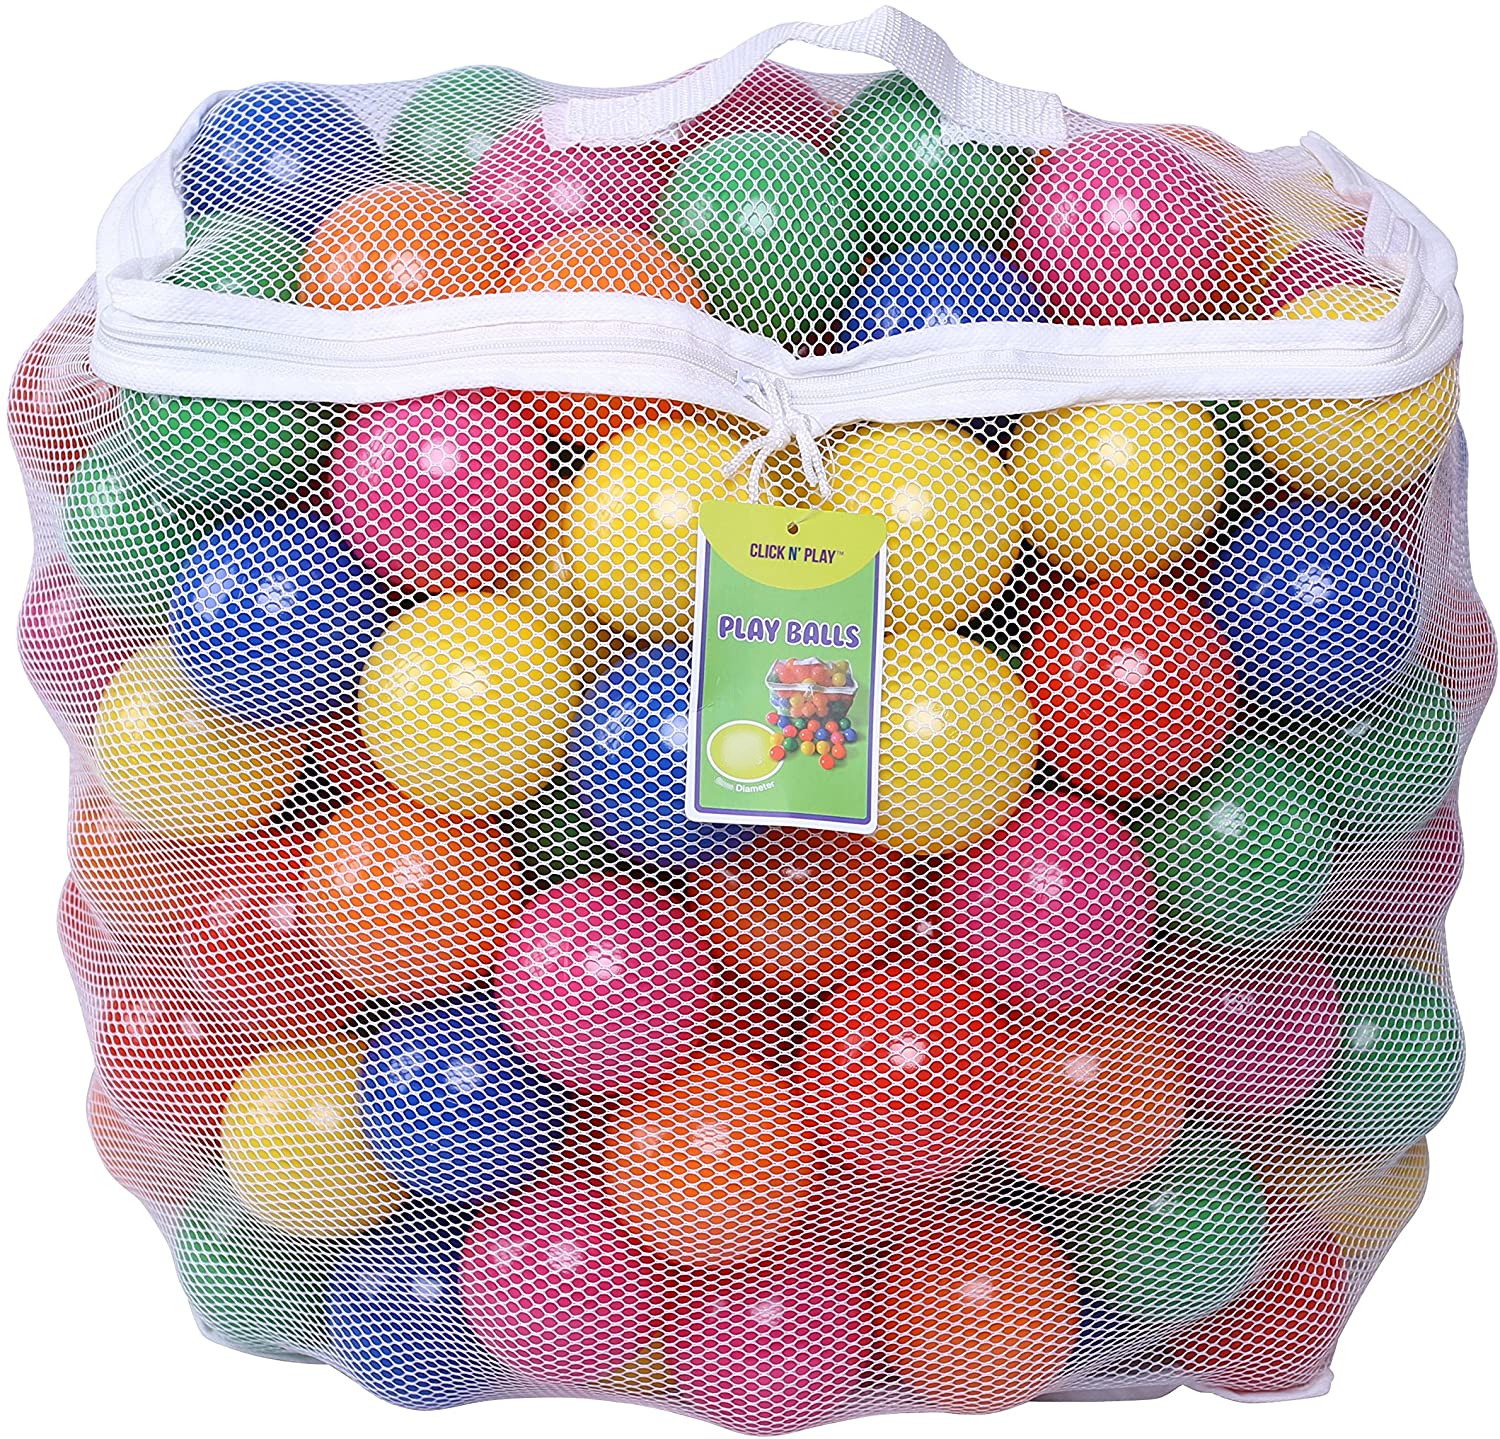
\includegraphics[width=3in]{ballsInBag.jpg}
  \end{center}
  About how many play balls are in the bag?
  \begin{enumerate}
  \item around $50$
  \item around $100$
  \item around $200$
  \end{enumerate}
\end{exercise}


\begin{exercise}
  Suppose that every ball has a mass of $5$ grams.  What expression
  will best approximate the mass of the bag?
  \begin{enumerate}
  \item $(\text{total number of balls})\times5$
  \item $(\text{total number of balls})\times25$
  \item $(\text{total number of balls})\times125$
  \end{enumerate}
\end{exercise}


\begin{exercise}
  Suppose they make a bag of \textit{Play Time Happy Fun Balls} where
  every linear dimension of the bag is scaled by a factor $2$.

  
  \textbf{How many more play balls are in this larger bag?}
  \begin{multicols}{2}
  \begin{enumerate}
  \item Half as many.
  \item Twice as many.
  \item Four times as many.
  \item Six times as many.
  \item Eight times as many.
  \item Sixteen times as many.
  \end{enumerate}
  \end{multicols}
\end{exercise}



\begin{exercise}
 Suppose they make a bag of \textit{Play Time Happy Fun Balls} where
  every linear dimension of the bag is scaled by a factor $2$.

  
  \textbf{How much longer will the zipper be (at the top of the bag)
    to access the balls?}
  \begin{multicols}{2}
  \begin{enumerate}
  \item Half as long.
  \item Twice as long.
  \item Four times as long.
  \item Six times as long.
  \item Eight times as long.
  \item Sixteen times as long.
  \end{enumerate}
  \end{multicols}
\end{exercise}



\begin{exercise}
  Suppose they make a bag of \textit{Play Time Happy Fun Balls} where
  every linear dimension of the bag is scaled by a factor $2$.

  
  \textbf{How much more fabric is required to make the bag?}
  \begin{multicols}{2}
    \begin{enumerate}
    \item Half as much.
    \item Twice as much.
    \item Four times as much.
    \item Six times as much.
    \item Eight times as much.
    \item Sixteen times as much.
    \end{enumerate}
  \end{multicols}
\end{exercise}




\answerlistbox{(c)}{(a)}{(e)}{(b)}{(c)}
\end{document}
